
%% bare_conf.tex
%% V1.3
%% 2007/01/11
%% by Michael Shell
%% See:
%% http://www.michaelshell.org/
%% for current contact information.
%%
%% This is a skeleton file demonstrating the use of IEEEtran.cls
%% (requires IEEEtran.cls version 1.7 or later) with an IEEE conference paper.
%%
%% Support sites:
%% http://www.michaelshell.org/tex/ieeetran/
%% http://www.ctan.org/tex-archive/macros/latex/contrib/IEEEtran/
%% and
%% http://www.ieee.org/

%%*************************************************************************
%% Legal Notice:
%% This code is offered as-is without any warranty either expressed or
%% implied; without even the implied warranty of MERCHANTABILITY or
%% FITNESS FOR A PARTICULAR PURPOSE! 
%% User assumes all risk.
%% In no event shall IEEE or any contributor to this code be liable for
%% any damages or losses, including, but not limited to, incidental,
%% consequential, or any other damages, resulting from the use or misuse
%% of any information contained here.
%%
%% All comments are the opinions of their respective authors and are not
%% necessarily endorsed by the IEEE.
%%
%% This work is distributed under the LaTeX Project Public License (LPPL)
%% ( http://www.latex-project.org/ ) version 1.3, and may be freely used,
%% distributed and modified. A copy of the LPPL, version 1.3, is included
%% in the base LaTeX documentation of all distributions of LaTeX released
%% 2003/12/01 or later.
%% Retain all contribution notices and credits.
%% ** Modified files should be clearly indicated as such, including  **
%% ** renaming them and changing author support contact information. **
%%
%% File list of work: IEEEtran.cls, IEEEtran_HOWTO.pdf, bare_adv.tex,
%%                    bare_conf.tex, bare_jrnl.tex, bare_jrnl_compsoc.tex
%%*************************************************************************

% *** Authors should verify (and, if needed, correct) their LaTeX system  ***
% *** with the testflow diagnostic prior to trusting their LaTeX platform ***
% *** with production work. IEEE's font choices can trigger bugs that do  ***
% *** not appear when using other class files.                            ***
% The testflow support page is at:
% http://www.michaelshell.org/tex/testflow/



% Note that the a4paper option is mainly intended so that authors in
% countries using A4 can easily print to A4 and see how their papers will
% look in print - the typesetting of the document will not typically be
% affected with changes in paper size (but the bottom and side margins will).
% Use the testflow package mentioned above to verify correct handling of
% both paper sizes by the user's LaTeX system.
%
% Also note that the "draftcls" or "draftclsnofoot", not "draft", option
% should be used if it is desired that the figures are to be displayed in
% draft mode.
%
\documentclass[10pt, conference, compsocconf]{IEEEtran}
% Add the compsocconf option for Computer Society conferences.
%
% If IEEEtran.cls has not been installed into the LaTeX system files,
% manually specify the path to it like:
% \documentclass[conference]{../sty/IEEEtran}





% Some very useful LaTeX packages include:
% (uncomment the ones you want to load)


% *** MISC UTILITY PACKAGES ***
%
\usepackage{ifpdf}
% Heiko Oberdiek's ifpdf.sty is very useful if you need conditional
% compilation based on whether the output is pdf or dvi.
% usage:
% \ifpdf
%   % pdf code
% \else
%   % dvi code
% \fi
% The latest version of ifpdf.sty can be obtained from:
% http://www.ctan.org/tex-archive/macros/latex/contrib/oberdiek/
% Also, note that IEEEtran.cls V1.7 and later provides a builtin
% \ifCLASSINFOpdf conditional that works the same way.
% When switching from latex to pdflatex and vice-versa, the compiler may
% have to be run twice to clear warning/error messages.






% *** CITATION PACKAGES ***
%
\usepackage{cite}
% cite.sty was written by Donald Arseneau
% V1.6 and later of IEEEtran pre-defines the format of the cite.sty package
% \cite{} output to follow that of IEEE. Loading the cite package will
% result in citation numbers being automatically sorted and properly
% "compressed/ranged". e.g., [1], [9], [2], [7], [5], [6] without using
% cite.sty will become [1], [2], [5]--[7], [9] using cite.sty. cite.sty's
% \cite will automatically add leading space, if needed. Use cite.sty's
% noadjust option (cite.sty V3.8 and later) if you want to turn this off.
% cite.sty is already installed on most LaTeX systems. Be sure and use
% version 4.0 (2003-05-27) and later if using hyperref.sty. cite.sty does
% not currently provide for hyperlinked citations.
% The latest version can be obtained at:
% http://www.ctan.org/tex-archive/macros/latex/contrib/cite/
% The documentation is contained in the cite.sty file itself.






% *** GRAPHICS RELATED PACKAGES ***
%
\ifCLASSINFOpdf
  \usepackage[pdftex]{graphicx}
  % declare the path(s) where your graphic files are
  % \graphicspath{{../pdf/}{../jpeg/}}
  % and their extensions so you won't have to specify these with
  % every instance of \includegraphics
  % \DeclareGraphicsExtensions{.pdf,.jpeg,.png}
\else
  % or other class option (dvipsone, dvipdf, if not using dvips). graphicx
  % will default to the driver specified in the system graphics.cfg if no
  % driver is specified.
  \usepackage[dvips]{graphicx}
  % declare the path(s) where your graphic files are
  % \graphicspath{{../eps/}}
  % and their extensions so you won't have to specify these with
  % every instance of \includegraphics
  % \DeclareGraphicsExtensions{.eps}
\fi
% graphicx was written by David Carlisle and Sebastian Rahtz. It is
% required if you want graphics, photos, etc. graphicx.sty is already
% installed on most LaTeX systems. The latest version and documentation can
% be obtained at: 
% http://www.ctan.org/tex-archive/macros/latex/required/graphics/
% Another good source of documentation is "Using Imported Graphics in
% LaTeX2e" by Keith Reckdahl which can be found as epslatex.ps or
% epslatex.pdf at: http://www.ctan.org/tex-archive/info/
%
% latex, and pdflatex in dvi mode, support graphics in encapsulated
% postscript (.eps) format. pdflatex in pdf mode supports graphics
% in .pdf, .jpeg, .png and .mps (metapost) formats. Users should ensure
% that all non-photo figures use a vector format (.eps, .pdf, .mps) and
% not a bitmapped formats (.jpeg, .png). IEEE frowns on bitmapped formats
% which can result in "jaggedy"/blurry rendering of lines and letters as
% well as large increases in file sizes.
%
% You can find documentation about the pdfTeX application at:
% http://www.tug.org/applications/pdftex





% *** MATH PACKAGES ***
%
\usepackage[cmex10]{amsmath}
% A popular package from the American Mathematical Society that provides
% many useful and powerful commands for dealing with mathematics. If using
% it, be sure to load this package with the cmex10 option to ensure that
% only type 1 fonts will utilized at all point sizes. Without this option,
% it is possible that some math symbols, particularly those within
% footnotes, will be rendered in bitmap form which will result in a
% document that can not be IEEE Xplore compliant!
%
% Also, note that the amsmath package sets \interdisplaylinepenalty to 10000
% thus preventing page breaks from occurring within multiline equations. Use:
%\interdisplaylinepenalty=2500
% after loading amsmath to restore such page breaks as IEEEtran.cls normally
% does. amsmath.sty is already installed on most LaTeX systems. The latest
% version and documentation can be obtained at:
% http://www.ctan.org/tex-archive/macros/latex/required/amslatex/math/





% *** SPECIALIZED LIST PACKAGES ***
%
\usepackage{algorithmic}
% algorithmic.sty was written by Peter Williams and Rogerio Brito.
% This package provides an algorithmic environment fo describing algorithms.
% You can use the algorithmic environment in-text or within a figure
% environment to provide for a floating algorithm. Do NOT use the algorithm
% floating environment provided by algorithm.sty (by the same authors) or
% algorithm2e.sty (by Christophe Fiorio) as IEEE does not use dedicated
% algorithm float types and packages that provide these will not provide
% correct IEEE style captions. The latest version and documentation of
% algorithmic.sty can be obtained at:
% http://www.ctan.org/tex-archive/macros/latex/contrib/algorithms/
% There is also a support site at:
% http://algorithms.berlios.de/index.html
% Also of interest may be the (relatively newer and more customizable)
% algorithmicx.sty package by Szasz Janos:
% http://www.ctan.org/tex-archive/macros/latex/contrib/algorithmicx/




% *** ALIGNMENT PACKAGES ***
%
\usepackage{array}
% Frank Mittelbach's and David Carlisle's array.sty patches and improves
% the standard LaTeX2e array and tabular environments to provide better
% appearance and additional user controls. As the default LaTeX2e table
% generation code is lacking to the point of almost being broken with
% respect to the quality of the end results, all users are strongly
% advised to use an enhanced (at the very least that provided by array.sty)
% set of table tools. array.sty is already installed on most systems. The
% latest version and documentation can be obtained at:
% http://www.ctan.org/tex-archive/macros/latex/required/tools/


\usepackage{mdwmath}
\usepackage{mdwtab}
% Also highly recommended is Mark Wooding's extremely powerful MDW tools,
% especially mdwmath.sty and mdwtab.sty which are used to format equations
% and tables, respectively. The MDWtools set is already installed on most
% LaTeX systems. The lastest version and documentation is available at:
% http://www.ctan.org/tex-archive/macros/latex/contrib/mdwtools/


% IEEEtran contains the IEEEeqnarray family of commands that can be used to
% generate multiline equations as well as matrices, tables, etc., of high
% quality.


\usepackage{eqparbox}
% Also of notable interest is Scott Pakin's eqparbox package for creating
% (automatically sized) equal width boxes - aka "natural width parboxes".
% Available at:
% http://www.ctan.org/tex-archive/macros/latex/contrib/eqparbox/





% *** SUBFIGURE PACKAGES ***
\usepackage[tight,footnotesize]{subfigure}
% subfigure.sty was written by Steven Douglas Cochran. This package makes it
% easy to put subfigures in your figures. e.g., "Figure 1a and 1b". For IEEE
% work, it is a good idea to load it with the tight package option to reduce
% the amount of white space around the subfigures. subfigure.sty is already
% installed on most LaTeX systems. The latest version and documentation can
% be obtained at:
% http://www.ctan.org/tex-archive/obsolete/macros/latex/contrib/subfigure/
% subfigure.sty has been superceeded by subfig.sty.



%\usepackage[caption=false]{caption}
%\usepackage[font=footnotesize]{subfig}
% subfig.sty, also written by Steven Douglas Cochran, is the modern
% replacement for subfigure.sty. However, subfig.sty requires and
% automatically loads Axel Sommerfeldt's caption.sty which will override
% IEEEtran.cls handling of captions and this will result in nonIEEE style
% figure/table captions. To prevent this problem, be sure and preload
% caption.sty with its "caption=false" package option. This is will preserve
% IEEEtran.cls handing of captions. Version 1.3 (2005/06/28) and later 
% (recommended due to many improvements over 1.2) of subfig.sty supports
% the caption=false option directly:
%\usepackage[caption=false,font=footnotesize]{subfig}
%
% The latest version and documentation can be obtained at:
% http://www.ctan.org/tex-archive/macros/latex/contrib/subfig/
% The latest version and documentation of caption.sty can be obtained at:
% http://www.ctan.org/tex-archive/macros/latex/contrib/caption/



% *** FLOAT PACKAGES ***
%
\usepackage{fixltx2e}
% fixltx2e, the successor to the earlier fix2col.sty, was written by
% Frank Mittelbach and David Carlisle. This package corrects a few problems
% in the LaTeX2e kernel, the most notable of which is that in current
% LaTeX2e releases, the ordering of single and double column floats is not
% guaranteed to be preserved. Thus, an unpatched LaTeX2e can allow a
% single column figure to be placed prior to an earlier double column
% figure. The latest version and documentation can be found at:
% http://www.ctan.org/tex-archive/macros/latex/base/



\usepackage{stfloats}
% stfloats.sty was written by Sigitas Tolusis. This package gives LaTeX2e
% the ability to do double column floats at the bottom of the page as well
% as the top. (e.g., "\begin{figure*}[!b]" is not normally possible in
% LaTeX2e). It also provides a command:
%\fnbelowfloat
% to enable the placement of footnotes below bottom floats (the standard
% LaTeX2e kernel puts them above bottom floats). This is an invasive package
% which rewrites many portions of the LaTeX2e float routines. It may not work
% with other packages that modify the LaTeX2e float routines. The latest
% version and documentation can be obtained at:
% http://www.ctan.org/tex-archive/macros/latex/contrib/sttools/
% Documentation is contained in the stfloats.sty comments as well as in the
% presfull.pdf file. Do not use the stfloats baselinefloat ability as IEEE
% does not allow \baselineskip to stretch. Authors submitting work to the
% IEEE should note that IEEE rarely uses double column equations and
% that authors should try to avoid such use. Do not be tempted to use the
% cuted.sty or midfloat.sty packages (also by Sigitas Tolusis) as IEEE does
% not format its papers in such ways.





% *** PDF, URL AND HYPERLINK PACKAGES ***
%
\usepackage{url}
% url.sty was written by Donald Arseneau. It provides better support for
% handling and breaking URLs. url.sty is already installed on most LaTeX
% systems. The latest version can be obtained at:
% http://www.ctan.org/tex-archive/macros/latex/contrib/misc/
% Read the url.sty source comments for usage information. Basically,
% \url{my_url_here}.

\usepackage{booktabs}



% *** Do not adjust lengths that control margins, column widths, etc. ***
% *** Do not use packages that alter fonts (such as pslatex).         ***
% There should be no need to do such things with IEEEtran.cls V1.6 and later.
% (Unless specifically asked to do so by the journal or conference you plan
% to submit to, of course. )


% correct bad hyphenation here
\hyphenation{op-tical net-works semi-conduc-tor}


\begin{document}
%
% paper title
% can use linebreaks \\ within to get better formatting as desired
\title{Facial expression recognition based on facial action unit}


% author names and affiliations
% use a multiple column layout for up to two different
% affiliations

\author{\IEEEauthorblockN{Jiannan Yang}
\IEEEauthorblockA{Computer Science and Technology \\
	Nanjing Tech University \\
	Jiangsu Province, China \\
	201861120038@njtech.edu.cn}
\and
\IEEEauthorblockN{Fan Zhang}
\IEEEauthorblockA{IBM Watson Group \\
	IBM Massachusette Lab \\
	Littleton, MA\\
	fzhang@us.ibm.com}
\and
\IEEEauthorblockN{Bike Chen}
\IEEEauthorblockA{Xinktech \\
	Building 22, No. -02, Xuanwu Avenue \\
	Jiangsu Province, China \\
	chenbike@xinktech.com}
\and
\IEEEauthorblockN{Samee U. Khan}
\IEEEauthorblockA{Electrical and Computer Eng \\
	North Dakota State Univ \\
	Fargo, ND \\
	samee.khan@ndsu.edu}
}
% conference papers do not typically use \thanks and this command
% is locked out in conference mode. If really needed, such as for
% the acknowledgment of grants, issue a \IEEEoverridecommandlockouts
% after \documentclass

% for over three affiliations, or if they all won't fit within the width
% of the page, use this alternative format:
% 
%\author{\IEEEauthorblockN{Michael Shell\IEEEauthorrefmark{1},
%Homer Simpson\IEEEauthorrefmark{2},
%James Kirk\IEEEauthorrefmark{3}, 
%Montgomery Scott\IEEEauthorrefmark{3} and
%Eldon Tyrell\IEEEauthorrefmark{4}}
%\IEEEauthorblockA{\IEEEauthorrefmark{1}School of Electrical and Computer Engineering\\
%Georgia Institute of Technology,
%Atlanta, Georgia 30332--0250\\ Email: see http://www.michaelshell.org/contact.html}
%\IEEEauthorblockA{\IEEEauthorrefmark{2}Twentieth Century Fox, Springfield, USA\\
%Email: homer@thesimpsons.com}
%\IEEEauthorblockA{\IEEEauthorrefmark{3}Starfleet Academy, San Francisco, California 96678-2391\\
%Telephone: (800) 555--1212, Fax: (888) 555--1212}
%\IEEEauthorblockA{\IEEEauthorrefmark{4}Tyrell Inc., 123 Replicant Street, Los Angeles, California 90210--4321}}




% use for special paper notices
%\IEEEspecialpapernotice{(Invited Paper)}




% make the title area
\maketitle


\begin{abstract}
In the past few years, there has been increasing interest in the perception of human expressions and mental states by machines, and Facial Expression Recognition (FER) has attracted increasing attention. Facial Action Unit (AU) is an early proposed method to describe facial muscle movements, which can effectively reflect the changes in people's facial expressions. In this paper, we propose a high-performance facial expression recognition method based on facial action unit, which can run on low-configuration computer and realize video and real-time camera FER. Our method is mainly divided into two parts. In the first part, 68 facial landmarks and image Histograms of Oriented Gradients (HOG) are obtained, and the feature values of action units are calculated accordingly. The second part uses three classification methods to realize the mapping from AUs to FER. We have conducted many experiments on the popular human FER benchmark datasets (CK+ and Oulu\_CASIA) to demonstrate the effectiveness of our method.
\end{abstract}

\begin{IEEEkeywords}
facial expression recognition; facial action unit; facial landmark;

\end{IEEEkeywords}


% For peer review papers, you can put extra information on the cover
% page as needed:
% \ifCLASSOPTIONpeerreview
% \begin{center} \bfseries EDICS Category: 3-BBND \end{center}
% \fi
%
% For peerreview papers, this IEEEtran command inserts a page break and
% creates the second title. It will be ignored for other modes.
\IEEEpeerreviewmaketitle



\section{Introduction}
Intuitively, facial expression recognition recognizes basic human expressions\cite{Peter2009Computation} (e.g., surprise, sadness, happiness, disgust, anger, etc.) by processing and analyzing face image features. Moreover, the potential applications of facial expression recognition are very extensive, such as service industry, criminal investigation and interrogation, medical help\cite{Girard2013Social} and so on. Most methods of facial expression recognition are mainly divided into two steps: feature extraction and classification. Feature extraction mainly analyzes the face image and obtains the potential features of the image. Since different expressions have different facial expression characteristics, it is possible to obtain effective potential features for better classification.

Facial action unit is by studying the movement of facial muscles\cite{Hager1985A}, and a method of describing facial movement changes. In 1978, American psychologist Ekman Paul and Friesen\cite{friesen1978facial} developed Facial Action Coding System (FACS), the system for almost all the muscles of the facial expression behavior carried on the detailed classification, is the facial expression enjoys wide application in measurement technology, one of the most representative methods. Although action units can accurately express facial expressions, they are rarely used in facial expression recognition due to the difficulty in accurate positioning. Currently, more and more attention has been paid to the study of facial action units. In recent years, there have been many studies on the positioning and detection of AUs. Ding X\cite{Ding2013Facial} et al. proposed a method based on Cascade of Tasks to detect facial action units.Baltrusaitis\cite{Baltrusaitis2015Cross} et al. presented a real-time facial action unit intensity estimation and occurrence system based on appearance features (Histograms of Oriented Gradients) and geometric features (shape parameters and landmark locations). Based on the detection method of AUs proposed by Baltrusaitis et al., this paper puts forward a method of facial expression recognition using face action units, which can meet the requirements of low-configuration equipment. The main contributions of this paper are as follows:

We proposed a facial expression recognition based on facial action unit and used multiple classification methods to realize the mapping of AUs to facial expression.

The proposed method has relatively low requirements for computer configuration and does not rely on GPU devices. It can run on a notebook computer with i5-8300 processor and 8G of memory, and the recognition speed of each image is maintained at about 30ms. So our program can realize video and real-time camera facial expression recognition.

\begin{figure*}[h]
	\centering
	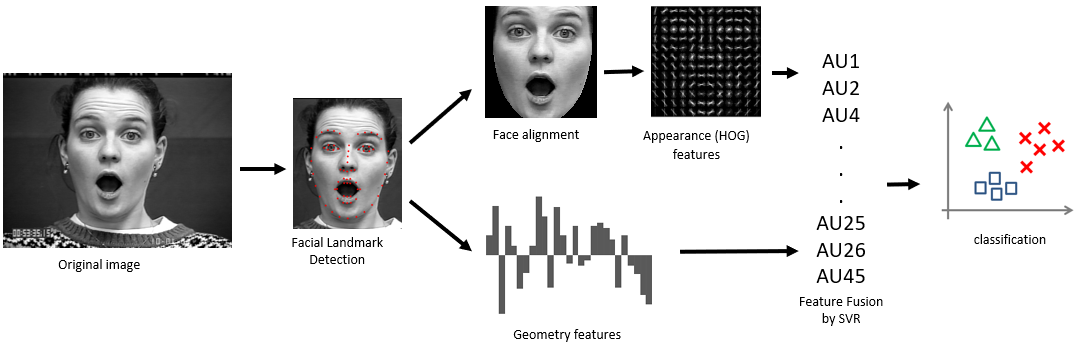
\includegraphics[width=\textwidth]{framework}
	\caption{Overview of facial expression recognition method based on facial action unit.}
\end{figure*}

\section{Related Work}

With the continuous improvement of computer performance, many more accurate facial expression recognition methods have been developed. In the past, traditional recognition methods have shown excellent performance in facial expression recognition. He\cite{He2005An} et al. proposed a facial expression recognition method based on classical LBP. Wang\cite{Wang2014Feature} et al. proposed a method of HOG and Weber Local Descriptor (WLD) feature fusion to realize facial expression recognition, in order to solve the problem of lack of contour and shape information. Berretti\cite{Berretti2010A} and others put forward a set of facial feature points calculation of depth image SIFT descriptors, and then select the most relevant feature subset of the original method.

With the advent of deep learning, facial expression recognition has been further developed. Liu\cite{Liu2017Adaptive} et al. proposed a generalized adaptive (N+M)-tuplet clusters loss function together with the identity-aware hard-negative mining and online positive mining scheme for facial expression recognition, which combined the deep metric loss and softmax loss in a unified two fully connected layer branches framework via joint optimization. Li\cite{li2018facial} et al.proposed a novel multi-scale CNN integrated with an attention-based learning layer (AMSCNN) for robust facial expression recognition. The attention-based learning layer is designed to automatically learn the importance of different receptive fields in the face during training. Meng\cite{Meng2017Identity} et al. developed an identity-aware convolutional neural network which utilizes identity information during the procedure of training model to alleviate variations introduced by personal attributes. In addition, contrastive loss and softmax loss are adopted jointly as supervision signals to optimize the neural network. Jung\cite{Jung2015Joint} et al. proposed a two branches deep neural network to do the task of FER, one of which extracts temporal appearance features from an image sequence, the other of which extracts temporal geometry features from temporal facial landmarks. Wu\cite{wu2018facial} et al. proposed a novel facial expression recognition method for different pose faces based on special landmark detection (FERMPI-SFL) to solve the problem that self-occlusion of facial posture will seriously affect the accuracy of facial expression recognition. 

\section{Proposed Method}
In this section, the detection methods of facial action units are first introduced, and then describe the three classification methods to realize the mapping of AUs to eight facial expressions (neutral, anger, contempt, happiness, disgust, sadness, fear and surprise). In the experiment, we extracted 16 AUs with prominent facial features. Figure 1 shows the detailed process of the method.

\subsection{Facial Action Unit}

We calculated 16 AUs with prominent facial features in the experiment. The description of AUs is shown in Table 1.

\begin{table}
	\caption{List of AUs.}
	\label{tab:freq}
	\centering
	\begin{tabular}{ccl}
		\toprule
		AU & Description & Example image\\ 
		\midrule
		1 & Inner Brow Raiser & \ \ \ \begin{minipage} {0.1\textwidth}   
			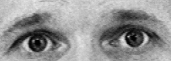
\includegraphics[width=0.6in]{AUimage/AU1.png}  
		\end{minipage}\\
		2 & Outer Brow Raiser & \ \ \ \begin{minipage} {0.1\textwidth}   
			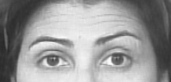
\includegraphics[width=0.6in]{AUimage/AU2.png}  
		\end{minipage}\\
		4 & Brow Lowererr & \ \ \ \begin{minipage} {0.1\textwidth}   
			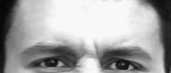
\includegraphics[width=0.6in]{AUimage/AU4.png}  
		\end{minipage}\\
		5 & Upper Lid Raiserr & \ \ \ \begin{minipage} {0.1\textwidth}   
			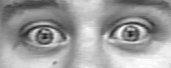
\includegraphics[width=0.6in]{AUimage/AU5.png}  
		\end{minipage}\\
		6 & Cheek Raiserr & \ \ \ \begin{minipage} {0.1\textwidth}   
			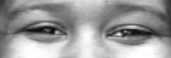
\includegraphics[width=0.6in]{AUimage/AU6.png}  
		\end{minipage}\\
		7 & Lid Tightenerr & \ \ \ \begin{minipage} {0.1\textwidth}   
			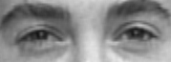
\includegraphics[width=0.6in]{AUimage/AU7.png}  
		\end{minipage}\\
		9 & Nose Wrinklerr & \ \ \ \begin{minipage} {0.1\textwidth}   
			
\includegraphics[width=0.6in]{AUimage/AU9.png}  
		\end{minipage}\\
		10 & Upper Lip Raiser & \ \ \ \begin{minipage} {0.1\textwidth}   
			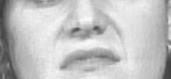
\includegraphics[width=0.6in]{AUimage/AU10.png}  
		\end{minipage}\\
		12 & Lip Corner Puller & \ \ \ \begin{minipage} {0.1\textwidth}   
			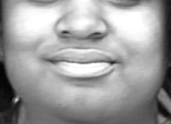
\includegraphics[width=0.6in]{AUimage/AU12.png}  
		\end{minipage}\\
		14 & Dimpler & \ \ \ \begin{minipage} {0.1\textwidth}   
			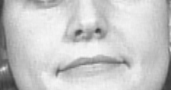
\includegraphics[width=0.6in]{AUimage/AU14.png}  
		\end{minipage}\\
		15 & Lip Corner Depressor & \ \ \ \begin{minipage} {0.1\textwidth}   
			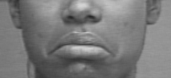
\includegraphics[width=0.6in]{AUimage/AU15.png}  
		\end{minipage}\\
		17 & Chin Raiser & \ \ \ \begin{minipage} {0.1\textwidth}   
			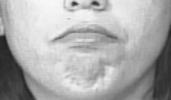
\includegraphics[width=0.6in]{AUimage/AU17.png}  
		\end{minipage}\\
		20 & Lip stretcher & \ \ \ \begin{minipage} {0.1\textwidth}   
			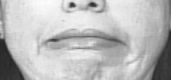
\includegraphics[width=0.6in]{AUimage/AU20.png}  
		\end{minipage}\\
		23 & Lip Tightener & \ \ \ \begin{minipage} {0.1\textwidth}   
			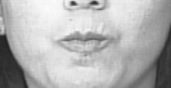
\includegraphics[width=0.6in]{AUimage/AU23.png}  
		\end{minipage}\\
		25 & Lips part & \ \ \ \begin{minipage} {0.1\textwidth}   
			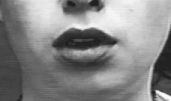
\includegraphics[width=0.6in]{AUimage/AU25.png}  
		\end{minipage}\\
		26 & Jaw Drop & \ \ \ \begin{minipage} {0.1\textwidth}   
			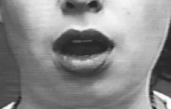
\includegraphics[width=0.6in]{AUimage/AU26.png}  
		\end{minipage}\\
		\bottomrule
	\end{tabular}
\end{table}
AU features extraction, using two main types of features: appearance features and geometric features. For appearance features, we get them by extracting direction gradient histogram. For geometric features, we rely on the coordinate results of the detection and tracking of facial landmark for the calculation of facial alignment. Here are the details.

For facial geometric features, Convolutional Experts Constrained Local Model (CE-CLM) proposed by Zadeh\cite{zadeh2017convolutional} et al. is used for the detection and analysis of facial landmark to obtain the coordinate positions. CE-CLM is an instance of Constrained Local Model (CLM)\cite{Cristinacce2006Feature}, It uses a local detector - Convolutional Experts Network (CEN) - that brings together the advantages of neural architectures and mixtures of experts in an end-to-end framework to optimize the results of CLM. We used CE-CLM model to mark 68 landmarks on the face as shown in Figure 2, which can clearly reflect the expression changes of various parts of the face (eyes, eyebrows, mouth, nose, etc.), and then we calculated the geometric features of the face image by comparing with the facial landmarks of the neutral expression. It is a difficult problem to standardize the landmarks of neutral expression because the facial landmarks of each person are not uniform. Therefore, we conduct a comparison based on dynamics, and we capture the geometric features of the face by training and learning the changes in the position of 68 landmarks. For the subsequent calculation of appearance features, we separated the face area and aligned it to fixed image size (112 $\times$ 112).

\begin{figure}[h]
	\centering
	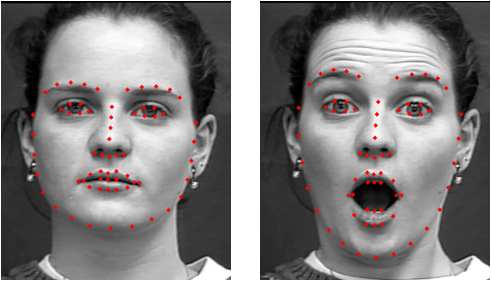
\includegraphics[width=\linewidth]{CECLM}
	\caption{The results of 68 landmarks in CE-CLM model are shown in the figure, neutral expression on the left and surprised expression on the right. The geometric features of the face are obtained by comparing the changes in the position of landmarks.}
\end{figure}

After face image alignment, we can extract appearance features, as the method proposed by Baltrusaitis\cite{Baltrusaitis2015Cross} et al. When extracting Histograms of Oriented Gradients (HOG), we use Principal Component Analysis (PCA) method to reduce the dimension of HOG feature vector, because we need to reduce the dimension to meet the problem of expression analysis.

Finally, we used support vector regression to estimate the intensity of AUs. Among them, we used a linear kernel to improve the training speed, because we were interested in real-time detection methods.

\subsection{Classification}
\par After obtaining the values of the AUs through the above method, We need to preprocess the AU values, formula (1) shows the method of processing AUs. Min-max Normalization is firstly used to normalize the values, avoid characteristic value is too large or too small. Then we will square the results, in order to make the features of the corresponding expression more outstanding, reduce the influences of other irrelevant features, and thus more accurate classification.

\begin{equation}\label{eqn:1}
\begin{split}
\displaystyle {AU_x}^{'} \ =\ \left(  \frac{AU_x\ -\ min\left\{\ AU_i\ \right\}} {max\left\{\ AU_i\ \right\}\ -\ min\left\{\ AU_i\ \right\}}\right)^2
\end{split}
\end{equation}
\par where, x is for every particular AU subscript, and i is for all the AU subscripts.
\par Then we combined AUs according to the changes of facial muscles corresponding to different expressions. Figure 3- Figure 9 show the changes in AUs corresponding to expressions.

\begin{figure}[h]
	\centering
	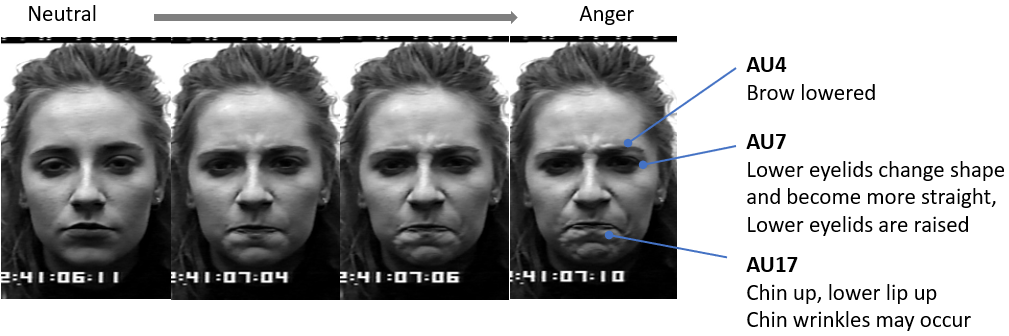
\includegraphics[width=\linewidth]{AUexpression/anger}
	\caption{The prominent changes of AUs corresponding to the anger expression.}
\end{figure}
\begin{figure}[h]
	\centering
	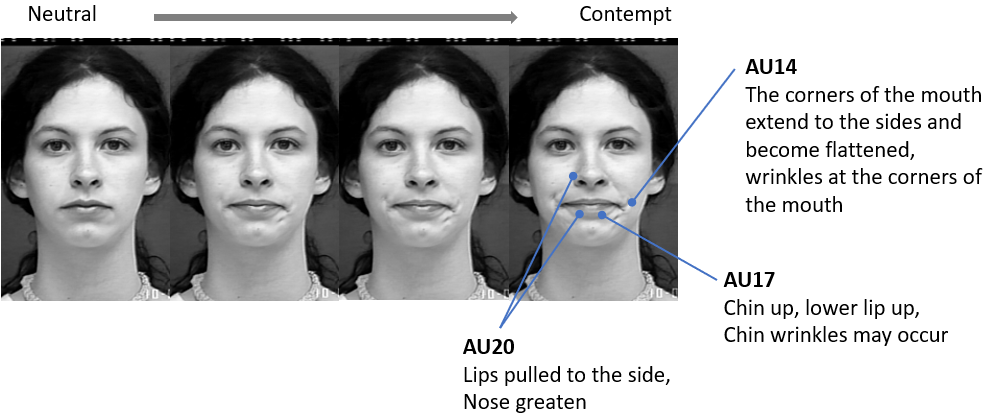
\includegraphics[width=\linewidth]{AUexpression/contempt}
	\caption{The prominent changes of AUs corresponding to the contempt expression.}
\end{figure}

From the figures, we can see that each expression triggers the movement of facial muscles, and the performance of each expression are basically similar, so we combined AUs for 7 expressions(not including neutral expression) to highlight the characteristics of the expression in the classification process. The results of the combinations are shown in Table 2. We get the characteristic values of the combination through the following formula:
\begin{equation}\label{eqn:1}
\begin{split}
\displaystyle AU_{E_k}\ =\ \lfloor\frac{2\sum AU_i^{'}}{\sum max_{2x}\{\ AU_j^{'}\ \} }\rfloor
\end{split}
\end{equation}
where, $E_k$ is  the k-th combination of the corresponding expression(E is the abbreviation of emotion), i is the subscript of AU in the combination, x is the number of AUs in each combination, j is for all subscripts of AUs, $max_{2x}$ means taking the maximum 2x values of AUs.

\begin{table}
	\caption{Expression-related AU combinations}
	\label{tab:freq}
	\begin{tabular}{ccl}
		\toprule
		\ \ \ \ \ \ \ \ Emotion\ \ \ \ \ \ \ \ & \ \ \ \ \ \ \ \ Combination of AUs\ \ \ \ \ \ \ \ \\
		\midrule
		Anger & 4+7+17, 4+5+7+23\\
		Contempt &14+17+20\\
		Disgust & 4+6+7+9, 7+9+10+17\\
		Fear & 1+2+20+25, 4+5+20\\
		Happiness & 6+7+12+25\\
		Sadness &1+4+15+17\\
		Surprise & 1+2+5+25+26\\
		\bottomrule
	\end{tabular}
\end{table}

\begin{figure}[h]
	\centering
	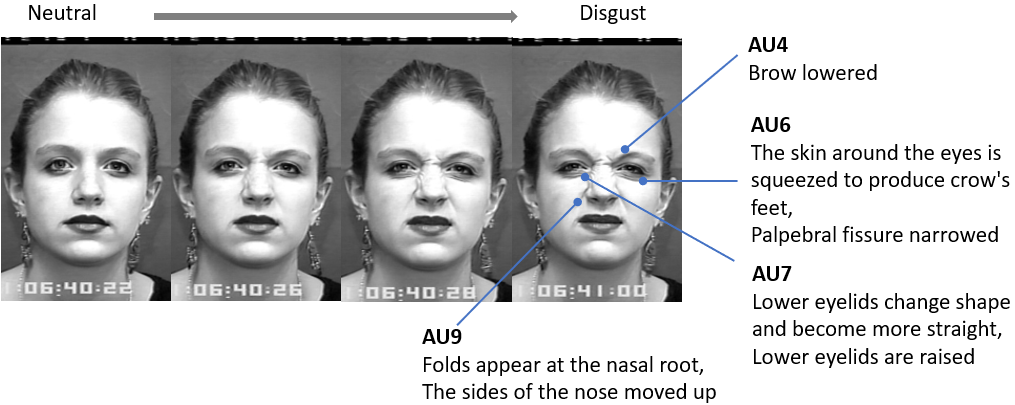
\includegraphics[width=\linewidth]{AUexpression/disgust}
	\caption{The prominent changes of AUs corresponding to the disgust expression.}
\end{figure}
\begin{figure}[h]
	\centering
	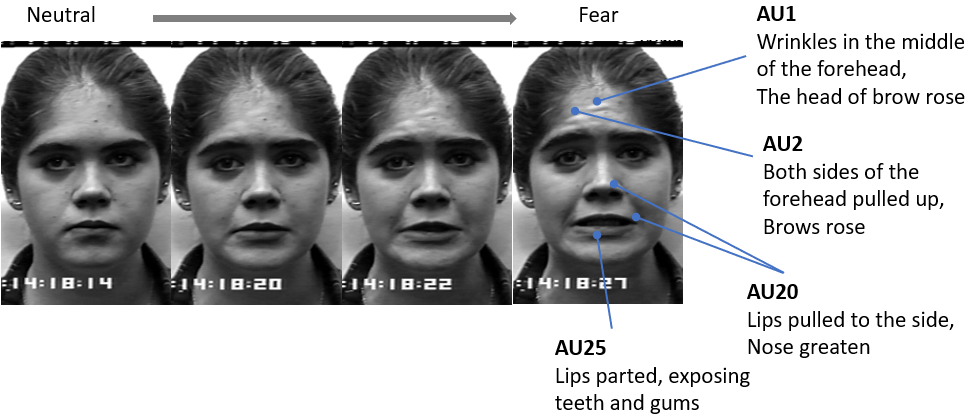
\includegraphics[width=\linewidth]{AUexpression/fear}
	\caption{The prominent changes of AUs corresponding to the fear expression.}
\end{figure}
\begin{figure}[h]
	\centering
	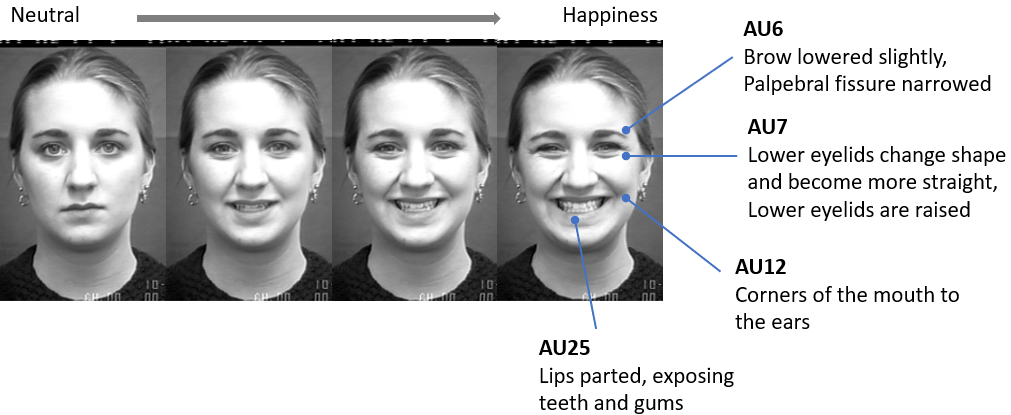
\includegraphics[width=\linewidth]{AUexpression/happiness}
	\caption{The prominent changes of AUs corresponding to the happy expression.}
\end{figure}
\begin{figure}[h]
	\centering
	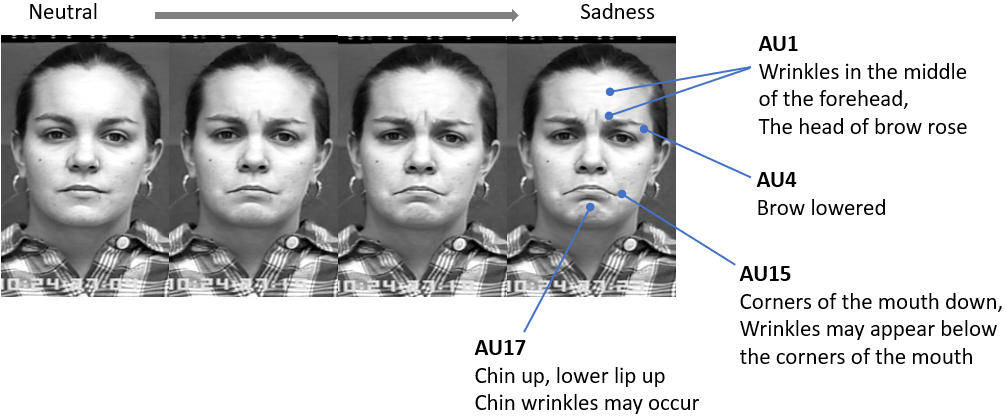
\includegraphics[width=\linewidth]{AUexpression/sadness}
	\caption{The prominent changes of AUs corresponding to the sad expression.}
\end{figure}
\begin{figure}[h]
	\centering
	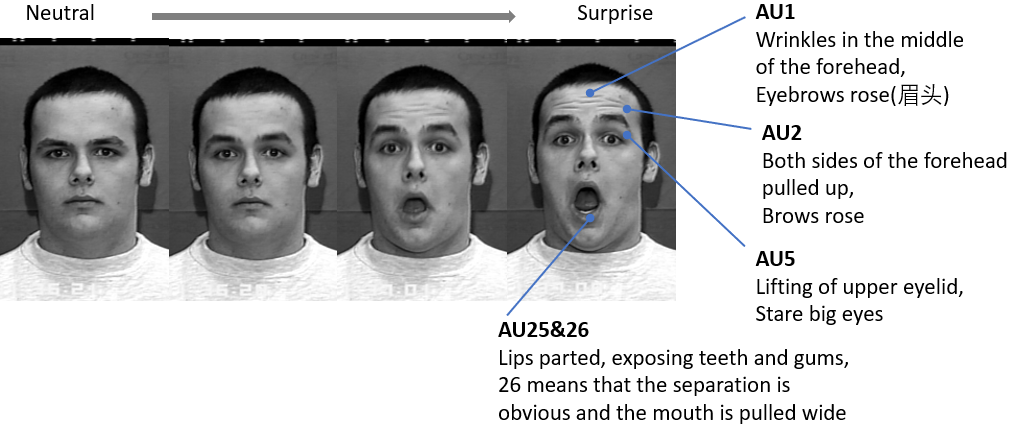
\includegraphics[width=\linewidth]{AUexpression/surprise}
	\caption{The prominent changes of AUs corresponding to the surprised expression.}
\end{figure}

Finally, we used three classification methods to achieve the mapping of AUs to eight expressions, namely Support Vector Machine (SVM), Extreme Gradient Boosting (Xgboost) and Deep Neural Networks (DNN). At the same time, we use 10-fold cross-validation for each method and compare the results of classification to verify the effectiveness of our method. For SVM, we used linear kernel for the kernel function, because it can effectively improve our computational efficiency and has little impact on the classification results. Meanwhile, we verified the penalty item C parameter of the SVM model during the training. We choose the gbtree model as booster parameter input, which uses the tree-based model for booster calculation in Xgboost. We use the deep neural network to build a simple classifier for classification, and design a three-layer neural network, which contains 10, 20, 10 neurons, the input layer are AU features, the output layer are eight basic expressions. Finally, we trained the neural network 30,00 times.

\section{Experiments}

\subsection{Dataset}

CK+ dataset: CK + dataset\cite{Lucey2010The} is composed of image sequences of eight expressions video recorded by 118 subjects. It is widely used to evaluate facial expression recognition methods. Each sequence in the dataset was marked with one of eight expression labels, such as neutral, anger, contempt, happiness, disgust, sadness, fear and surprise. The label is only provided for the last frame (called peak frame) of each image sequence. In order to obtain more experimental data, the dataset we trained contains the last 3-6 images (obvious facial expression features) of each image sequence, which is composed of 1492 images. We divide CK + dataset into 10 subsets, each of which is strictly independent of the principal. Data from eight subsets were used for training, and the remaining two were used for testing and validation, with 10-fold cross-validation used during training.

Oulu\_CASIA dataset: Oulu\_CASIA dataset\cite{Zhao2011Facial} consists of 80 subjects, each of which contains 6 basic expressions  (happiness, sadness, anger, fear, disgust, and surprise). Images of each facial expression are captured with two imaging systems: near-infrared (NIR) and visible light (VIS) under one of three different illumination conditions: normal indoor illumination, weak illumination, and dim illumination. Thence, Oulu\_CASIA dataset includes 2880 image sequences. Following the previous approaches evaluated on the Oulu\_CASIA dataset, only 480 image sequences taken under normal illumination conditions by VIS system are utilized in our experiments. The last three frames are collected as peak frames of the labeled expression. Thus, a total number of 1440 images in the Oulu\_CASIA dataset is used to evaluate our facial expression recognition system. Similar to the process utilized on CK+ dataset, we also split the Oulu\_CASIA dataset into 10 subsets and each of them is strictly subjected independent. Data from 8 subsets are employed for training and the remaining 2 subsets are adopted to validation and testing respectively. 10-fold cross-validation is also employed during the training.

\begin{figure}[h]
	\centering
	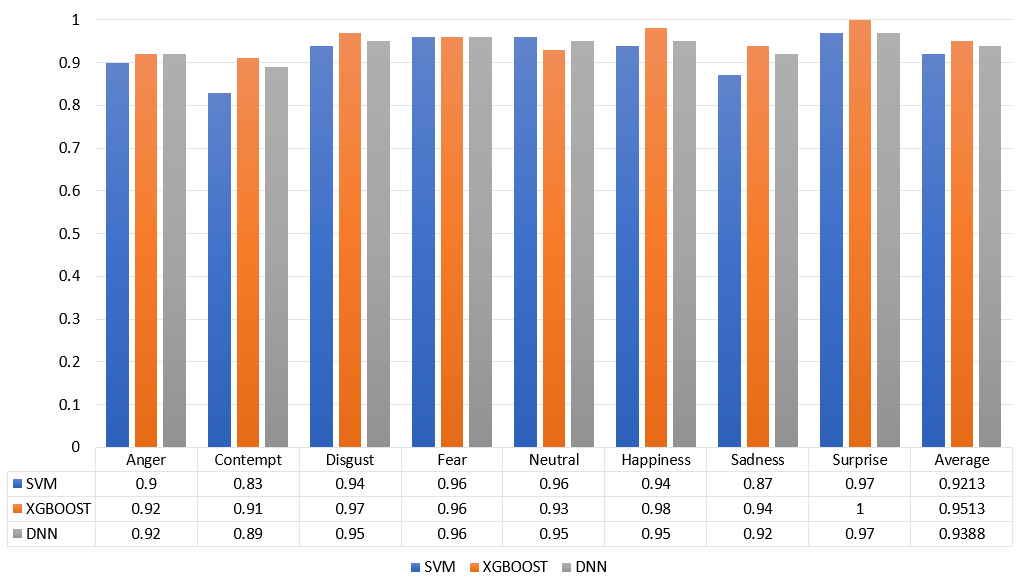
\includegraphics[width=\linewidth]{figureck}
	\caption{The recognition rate of AU combinations on different categories of facial expression on CK+ dataset.}
\end{figure}
\begin{figure}[h]
	\centering
	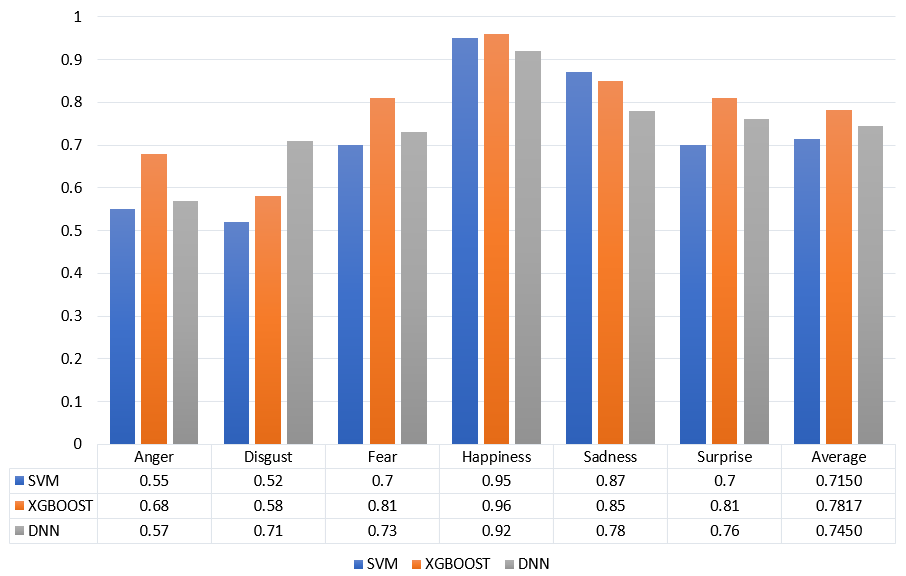
\includegraphics[width=\linewidth]{figureoulu}
	\caption{The recognition rate of AU combinations on different categories of facial expression on Oulu\_CASIA dataset.}
\end{figure}
\begin{figure}[h]
	\centering
	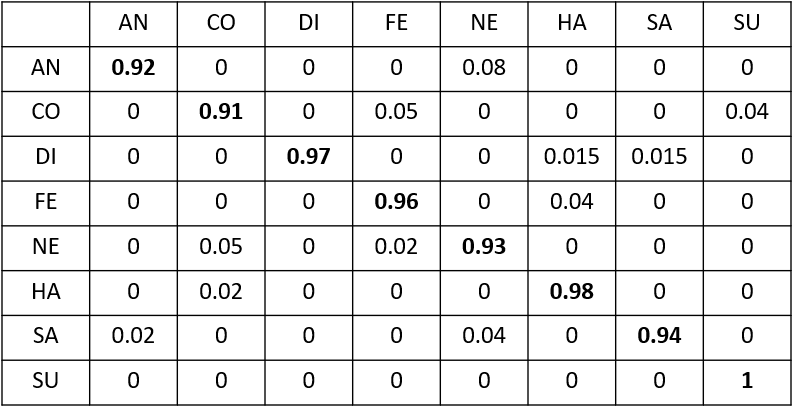
\includegraphics[width=\linewidth]{ConfusionmatrixCK}
	\caption{Confusion matrix of Xgboost classification method evaluated on the CK+ dataset(AN: angry, DI: disgust, HA: happiness, SA: sadness, SU: surprise, FE: fear, CO: contempt).}
\end{figure}
\begin{figure}[h]
	\centering
	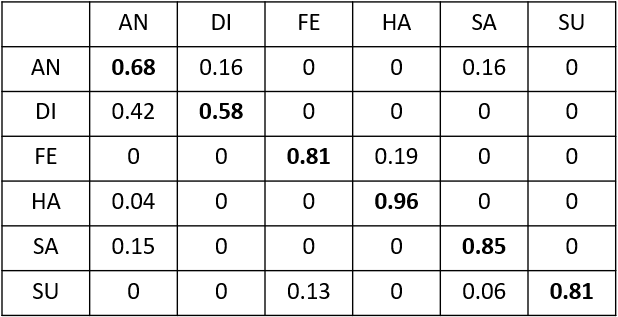
\includegraphics[width=\linewidth]{ConfusionmatrixOULU}
	\caption{Confusion matrix of Xgboost classification method evaluated on the Oulu\_CASIA dataset(AN: angry, DI: disgust, HA: happiness, SA: sadness, SU: surprise, FE: fear, CO: contempt).}
\end{figure}

\subsection{Result}

For the experimental evaluation, we compared the results of three different classification methods on two datasets. For the test set, we used about 40 separate images for each expression (not training), totaling 337 test images on CK+ dataset and totaling 240 test images on Oulu\_CASIA dataset. We calculated and counted the recognition accuracy of each expression, and calculated the average accuracy corresponding to the three methods. Figure 10 and Figure 11 show the details. Meanwhile, we list the confusion matrix of the Xgboost classification method on both datasets as shown in the Figure 12 and Figure 13.

It can be clearly seen that for CK+ dataset our methods achieved better results, especially the Xgboost classifier with higher accuracy. And for Oulu\_CASIA dataset, the average accuracy of all three methods is relatively low. For the two datasets, CK+'s images(640 $\times$ 490) are more clear and the expressions of people are more obvious. The position of human faces is relatively fixed, while the resolution of the images in Oulu\_CASIA dataset is relatively small, only 320 $\times$ 240, so the expressions are blurred. We realize expression recognition based on AUs mapping to expressions, and the accuracy of AU feature acquisition directly affects the final result. Therefore, our method requires relatively high qualities of pictures to obtain more accurate AU values, and clear pictures can often get more accurate results.

\begin{figure}
	\centering
	\begin{minipage}[c]{0.5\textwidth}
		\centering	
		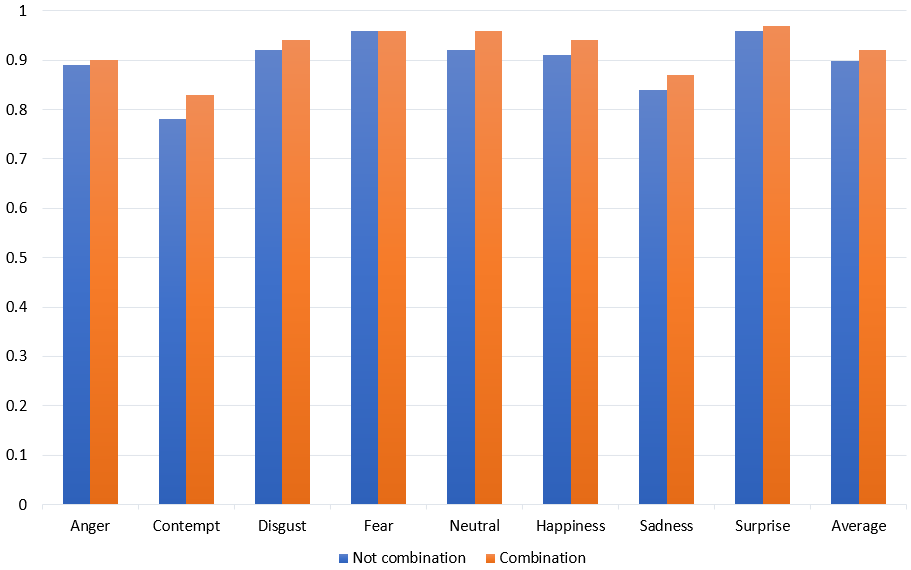
\includegraphics[height=4.5cm,width=7.5cm]{SVM}
	\end{minipage}
	( a )
	\begin{minipage}[c]{0.5\textwidth}
		\centering
		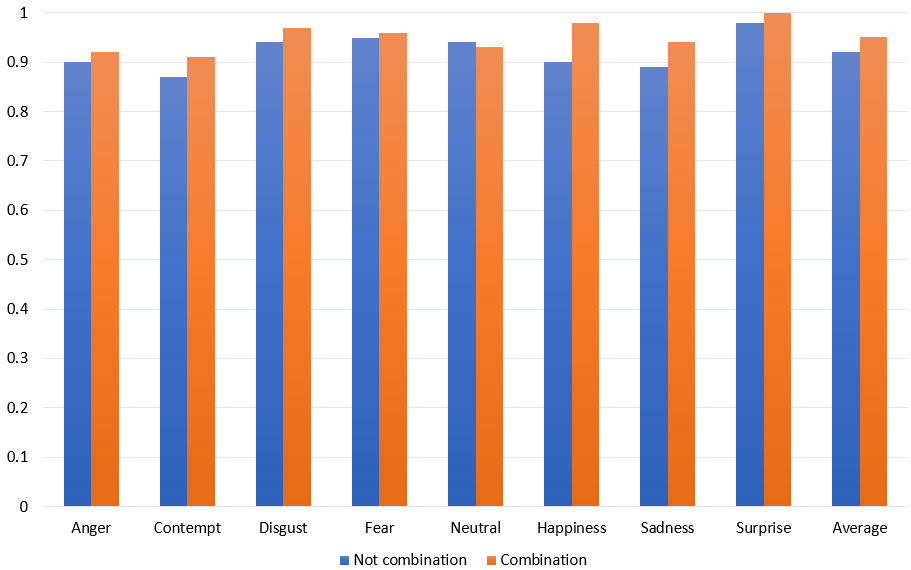
\includegraphics[height=4.5cm,width=7.5cm]{XGBOOST}	
	\end{minipage}
	( b )
	\begin{minipage}[c]{0.5\textwidth}
		\centering
		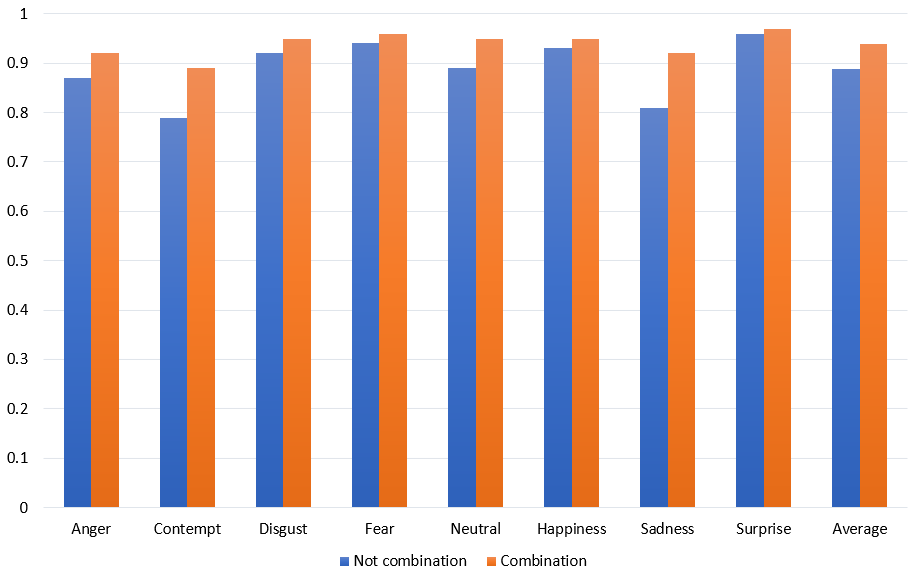
\includegraphics[height=4.5cm,width=7.5cm]{DNN}	
	\end{minipage}
	( c )
	\caption{Comparison of the experimental results after AU combinations and the results of original data directly used for classification on CK+ dataset, the three charts are respectively the classification results of (a) SVM, (b) XGBOOST and (c) DNN.}
\end{figure}

At the same time, we tested the real-time performance of facial expression recognition. We obtained face images through the camera, took each frame as the input image of the program, with size 640x480, and tested it in a noteBook computer with Intel i5-8300 processor and 8G of memory. We calculated the speed of facial expression recognition at about 30ms (33.3fps) through the input time of the image and the output time of the recognition result, and continuously output each frame  containing the classification result. This proves that our method can realize video or camera facial expression recognition in real time.

Finally, we verified the effectiveness of our AU combination method by comparing the experimental results before and after the combinations of AUs on CK+ dataset. Figure 14 shows the comparison results. It can be seen that the combinations of AUs have significantly improved the recognition results of each expression.

\section{Conclusion}

In this paper, the mapping from facial action unit to facial expression recognition is realized. Firstly, facial landmark detection and Histograms of Oriented Gradients are used to acquire facial action units according to facial appearance and geometric features, and then different classification methods are used to train and classify the above results, corresponding to eight kinds of expressions. Experiments are carried out on benchmark datasets (CK+ and Oulu\_CASIA) to verify the effectiveness of the application of facial action units in the field of facial expression recognition. With the development of technology, we hope to get facial action units more accurately and make it more widely used.


% An example of a floating figure using the graphicx package.
% Note that \label must occur AFTER (or within) \caption.
% For figures, \caption should occur after the \includegraphics.
% Note that IEEEtran v1.7 and later has special internal code that
% is designed to preserve the operation of \label within \caption
% even when the captionsoff option is in effect. However, because
% of issues like this, it may be the safest practice to put all your
% \label just after \caption rather than within \caption{}.
%
% Reminder: the "draftcls" or "draftclsnofoot", not "draft", class
% option should be used if it is desired that the figures are to be
% displayed while in draft mode.
%
%\begin{figure}[!t]
%\centering
%\includegraphics[width=2.5in]{myfigure}
% where an .eps filename suffix will be assumed under latex, 
% and a .pdf suffix will be assumed for pdflatex; or what has been declared
% via \DeclareGraphicsExtensions.
%\caption{Simulation Results}
%\label{fig_sim}
%\end{figure}

% Note that IEEE typically puts floats only at the top, even when this
% results in a large percentage of a column being occupied by floats.


% An example of a double column floating figure using two subfigures.
% (The subfig.sty package must be loaded for this to work.)
% The subfigure \label commands are set within each subfloat command, the
% \label for the overall figure must come after \caption.
% \hfil must be used as a separator to get equal spacing.
% The subfigure.sty package works much the same way, except \subfigure is
% used instead of \subfloat.
%
%\begin{figure*}[!t]
%\centerline{\subfloat[Case I]\includegraphics[width=2.5in]{subfigcase1}%
%\label{fig_first_case}}
%\hfil
%\subfloat[Case II]{\includegraphics[width=2.5in]{subfigcase2}%
%\label{fig_second_case}}}
%\caption{Simulation results}
%\label{fig_sim}
%\end{figure*}
%
% Note that often IEEE papers with subfigures do not employ subfigure
% captions (using the optional argument to \subfloat), but instead will
% reference/describe all of them (a), (b), etc., within the main caption.


% An example of a floating table. Note that, for IEEE style tables, the 
% \caption command should come BEFORE the table. Table text will default to
% \footnotesize as IEEE normally uses this smaller font for tables.
% The \label must come after \caption as always.
%
%\begin{table}[!t]
%% increase table row spacing, adjust to taste
%\renewcommand{\arraystretch}{1.3}
% if using array.sty, it might be a good idea to tweak the value of
% \extrarowheight as needed to properly center the text within the cells
%\caption{An Example of a Table}
%\label{table_example}
%\centering
%% Some packages, such as MDW tools, offer better commands for making tables
%% than the plain LaTeX2e tabular which is used here.
%\begin{tabular}{|c||c|}
%\hline
%One & Two\\
%\hline
%Three & Four\\
%\hline
%\end{tabular}
%\end{table}


% Note that IEEE does not put floats in the very first column - or typically
% anywhere on the first page for that matter. Also, in-text middle ("here")
% positioning is not used. Most IEEE journals/conferences use top floats
% exclusively. Note that, LaTeX2e, unlike IEEE journals/conferences, places
% footnotes above bottom floats. This can be corrected via the \fnbelowfloat
% command of the stfloats package.

% trigger a \newpage just before the given reference
% number - used to balance the columns on the last page
% adjust value as needed - may need to be readjusted if
% the document is modified later
%\IEEEtriggeratref{8}
% The "triggered" command can be changed if desired:
%\IEEEtriggercmd{\enlargethispage{-5in}}

% references section

% can use a bibliography generated by BibTeX as a .bbl file
% BibTeX documentation can be easily obtained at:
% http://www.ctan.org/tex-archive/biblio/bibtex/contrib/doc/
% The IEEEtran BibTeX style support page is at:
% http://www.michaelshell.org/tex/ieeetran/bibtex/
\bibliographystyle{IEEEtran}
% argument is your BibTeX string definitions and bibliography database(s)
%\bibliography{IEEEabrv,../bib/paper}
%
% <OR> manually copy in the resultant .bbl file
% set second argument of \begin to the number of references
% (used to reserve space for the reference number labels box)
\bibliography{reference}



% that's all folks
\end{document}


